\chapter{矢量分析基础}
在电磁理论中,我们要研究某些物理量在空间的分布和变化规律。为此,引入了\uwave{场}(Field)的概念。如果每一时刻,一个物理量在空间中的每一点都有一个确定的值,则称此空间中确定了该物理量的场。电磁场是三维空间的矢量场,因此,矢量分析是研究电磁场的重要数学工具。

\begin{itemize}
    \item 标量场在空间的变化规律,由其梯度描述。
    \item 矢量场在空间的变化规律,由其散度和旋度描述。
\end{itemize}
在本章,我们将首先复习矢量代数和正交坐标系,随后,重点讨论梯度、散度、旋度的定义及运算规律(高斯定理、斯托克斯定理),建立标量位和矢量位的概念,最后引出亥姆霍兹定理。

\section{矢量代数}
有关\uwave{标量}(Scalar)和\uwave{矢量}(Vector)的定义和矢量的一些基本性质,我们在高等数学中已经很熟悉了,这里不再赘述。这里重点复习一下矢量的两种乘法,即点积和叉积的定义和性质。

\subsection{矢量的点积}
\begin{BoxDefinition}[点积]
    矢量的\uwave{点积}(Dot Product)是一个标量,定义为
    \begin{Equation}
        \vb*{A}\cdot\vb*{B}=AB\cos\theta
    \end{Equation}
\end{BoxDefinition}
\begin{BoxProperty}[点积的性质]
    点积满足交换律
    \begin{Equation}
        \vb*{A}\cdot\vb*{B}=\vb*{B}\cdot\vb*{A}
    \end{Equation}
    点积满足分配律
    \begin{Equation}
        \vb*{A}\cdot(\vb*{B}+\vb*{C})=\vb*{A}\cdot\vb*{B}+\vb*{A}\cdot\vb*{C}
    \end{Equation}
\end{BoxProperty}

\subsection{矢量的叉积}
\begin{BoxDefinition}[叉积]
    矢量的\uwave{叉积}(Cross Product)是一个矢量,定义为
    \begin{Equation}
        \vb*{A}\times\vb*{B}=AB\sin\theta\vb*{e}_\text{n}
    \end{Equation}
    其中$\vb*{e}_n$是右手由矢量$\vb*{A}$选择至$\vb*{B}$时,大拇指的方向。
\end{BoxDefinition}
\begin{BoxProperty}[叉积的性质]
    叉积满足反交换律
    \begin{Equation}
        \vb*{A}\times\vb*{B}=-\vb*{B}\times\vb*{A}
    \end{Equation}
    叉积满足分配律
    \begin{Equation}
        \vb*{A}\times(\vb*{B}+\vb*{C})=\vb*{A}\times\vb*{B}+\vb*{A}\times\vb*{C}
    \end{Equation}
\end{BoxProperty}

\subsection{矢量的三重积}
矢量有点积和叉积两种“相乘”运算,因此当三个矢量“相乘”时,会出现两种三重积。\cite{W1}

\begin{BoxDefinition}[标量三重积]
    矢量$\vb*{A},\vb*{B},\vb*{C}$的\uwave{标量三重积}(Scalar Triple Product)被定义为
    \begin{Equation}
        \vb*{A}\cdot(\vb*{B}\times\vb*{C})
    \end{Equation}
\end{BoxDefinition}
\begin{BoxDefinition}[矢量三重积]
    矢量$\vb*{A},\vb*{B},\vb*{C}$的\uwave{矢量三重积}(Vector Triple Product)被定义为
    \begin{Equation}
        \vb*{A}\times(\vb*{B}\times\vb*{C})
    \end{Equation}
\end{BoxDefinition}

标量三重积比较重要的是下面的行列式表述
\begin{BoxFormula}[标量三重积的行列式表示]
    标量三重积可以表述为
    \begin{Equation}
        \vb*{A}\cdot\qty(\vb*{B}\times\vb*{C})=
        \begin{vmatrix}
            \vb*{A}\\
            \vb*{B}\\
            \vb*{C}\\
        \end{vmatrix}=
        \begin{vmatrix}
            A_x&A_y&A_z\\
            B_x&B_y&B_z\\
            C_x&C_y&C_z
        \end{vmatrix}
    \end{Equation}
\end{BoxFormula}

标量三重积具有很清楚的数学意义,它代表$\vb*{A},\vb*{B},\vb*{C}$围城的平行六面体的提及。

标量三重积具有轮换对称性,这就是说$\vb*{A},\vb*{B},\vb*{C}$和$\vb*{B},\vb*{C},\vb*{A}$和$\vb*{C},\vb*{A},\vb*{B}$的标量三重积其实是相同的,因为根据线性代数的知识,交换行列式的任意两行将会产生一个负号,而上述两两之间(对应行列式)的变换,均需要作两次行交换,产生的负号抵消,因而是相等的,即
\begin{BoxFormula}[标量三重积的轮换对称性]
    标量三重积具有轮换对称性
    \begin{Equation}
        \vb*{A}\cdot(\vb*{B}\times\vb*{C})=
        \vb*{B}\cdot(\vb*{C}\times\vb*{A})=
        \vb*{C}\cdot(\vb*{B}\times\vb*{A})
    \end{Equation}
\end{BoxFormula}
矢量三重积比较重要的,是下面的展开式
\begin{BoxFormula}[拉格朗日公式]
    矢量三重积具有以下展开式,称为\uwave{拉格朗日公式}(Lagrange Formula)
    \begin{Equation}
        \vb*{A}\times(\vb*{B}\times \vb*{C})=
        \vb*{B}(\vb*{A}\cdot\vb*{C})-
        \vb*{C}(\vb*{A}\cdot\vb*{B})
    \end{Equation}
\end{BoxFormula}
矢量三重积的展开公式可以“后面的出租车back cab”形象记忆,即BAC(K) CAB。

矢量三重积的一种变式是
\begin{Gather}[6pt]
    \vb*{A}\times(\vb*{B}\times \vb*{C})=
    \vb*{B}(\vb*{A}\cdot\vb*{C})-
    \vb*{C}(\vb*{A}\cdot\vb*{B})\\
    (\vb*{A}\times \vb*{B})\times\vb*{C}=
    \vb*{B}(\vb*{C}\cdot\vb*{A})-
    \vb*{A}(\vb*{C}\cdot\vb*{B})
\end{Gather}
如何同时记忆这两者呢,以下是一些诀窍
\begin{enumerate}
    \item 结果总是括号里那两个矢量的线性组合。
    \item 结果的线性组合中,原先位于中间的矢量(即$\vb*{B}$)的系数为正,另一矢量的系数为负。
    \item 矢量前的系数由另外两个矢量的点积构成,点积满足交换律,故这里的顺序不重要。
\end{enumerate}
矢量三重积的展开公式的一个直接结果是下面的恒等式
\begin{BoxFormula}[雅可比恒等式]
    矢量三重积满足以下恒等式,称为\uwave{雅可比恒等式}(Jacobi Identity)
    \begin{Equation}
        \vb*{A}\times(\vb*{B}\times \vb*{C})+\vb*{B}\times(\vb*{C}\times \vb*{A})+\vb*{C}\times(\vb*{A}\times \vb*{B})=\vb*{0}
    \end{Equation}
\end{BoxFormula}


\section{正交曲面坐标系}
在这一节,我们将首先通过我们最熟悉的直角坐标系,把握一般正交曲面坐标系中需要学习的要点,随后以此为基础,推演出柱坐标系和球坐标的相关属性,对比其与直角坐标系的不同。

\begin{Figure}[正交曲面坐标系]
    \begin{FigureSub}[柱坐标系]
        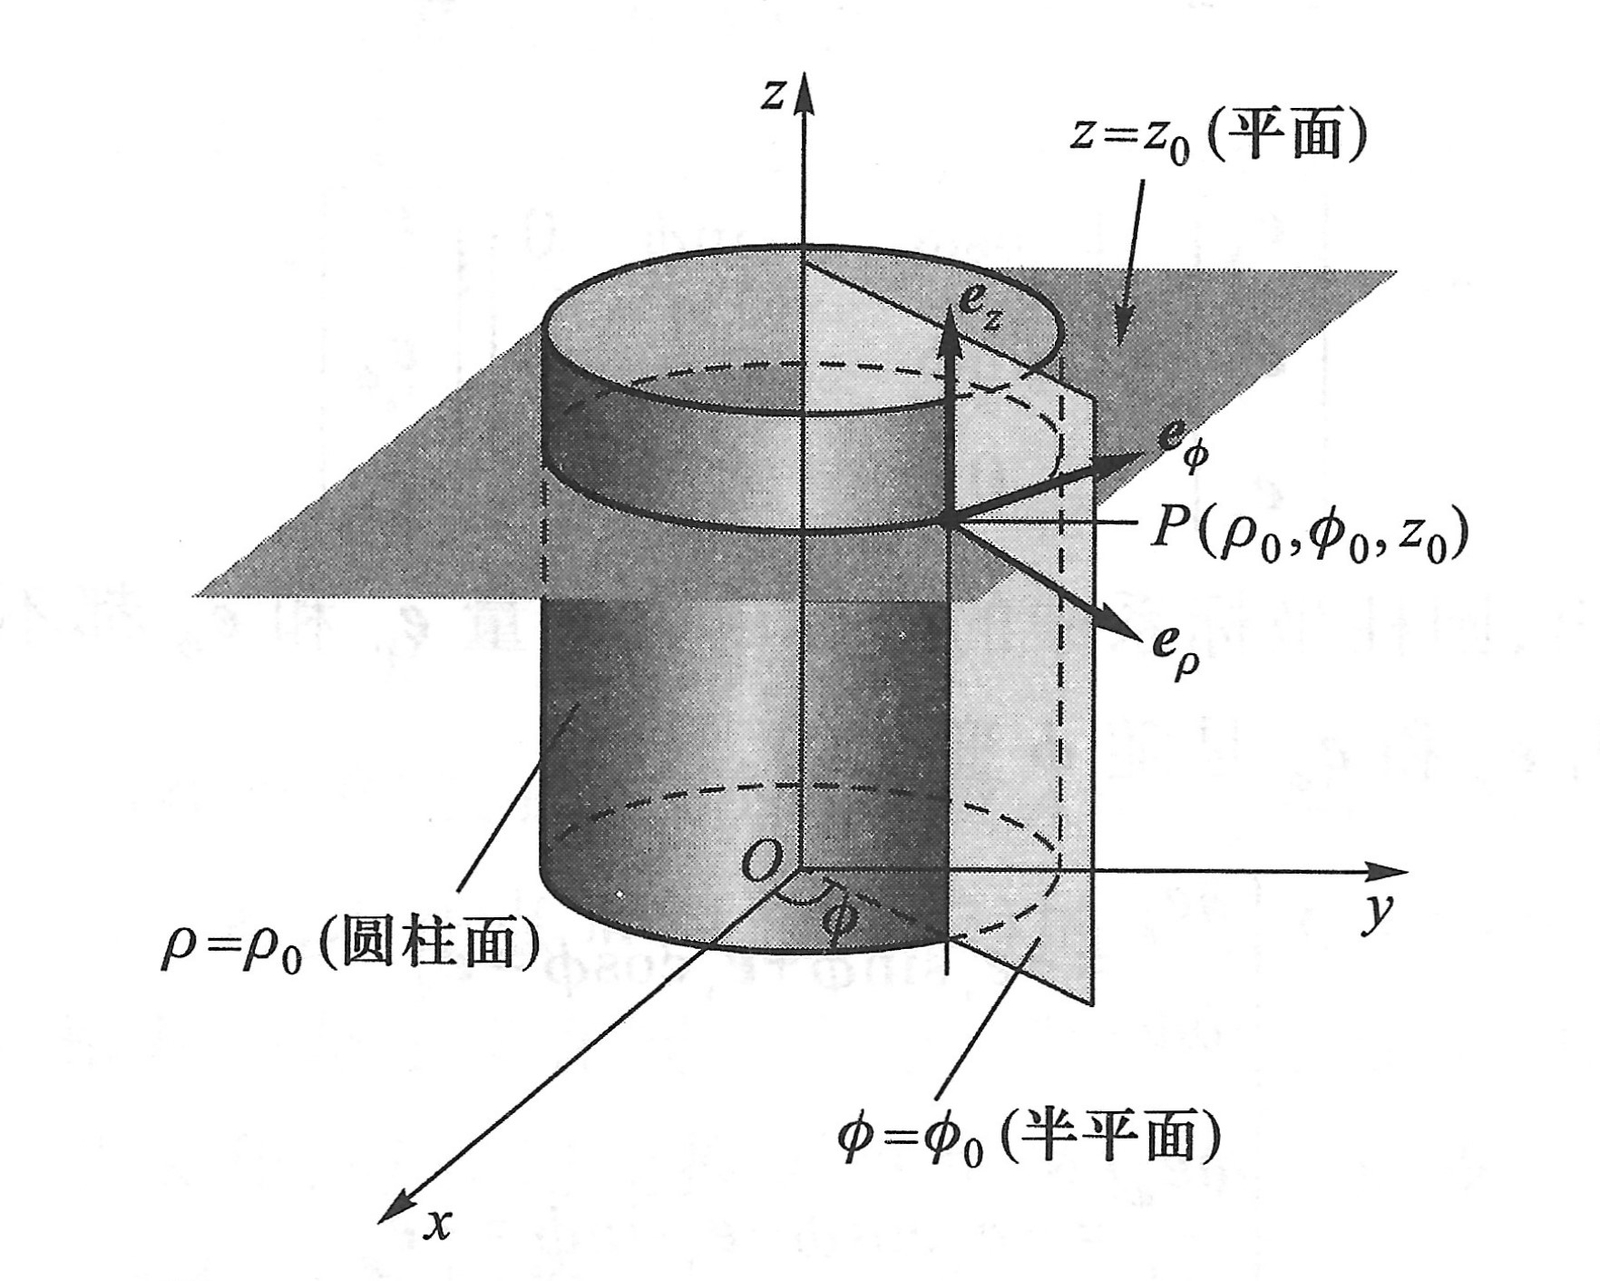
\includegraphics{image/1.jpg}
    \end{FigureSub}
    \begin{FigureSub}[球坐标系]
        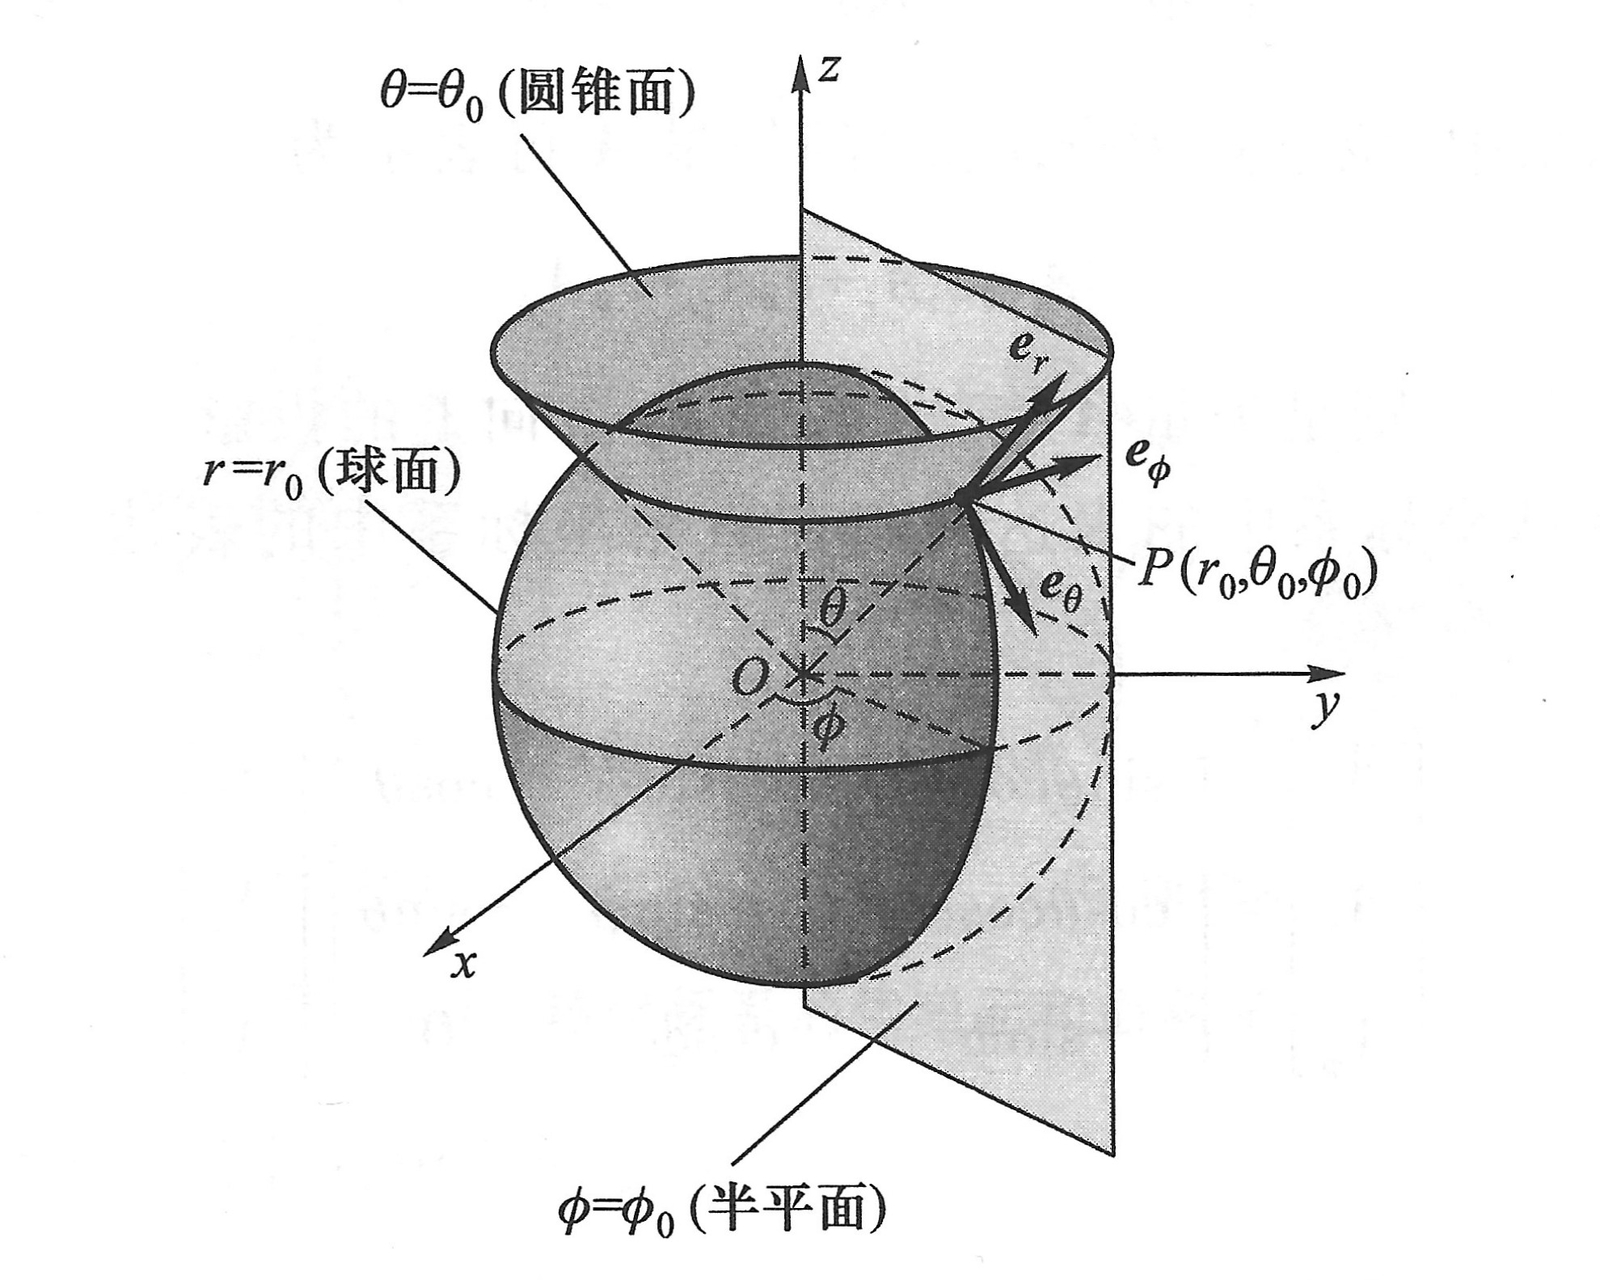
\includegraphics{image/2.jpg}
    \end{FigureSub}
\end{Figure}

\subsection{直角坐标系}
\begin{BoxDefinition}[直角坐标系]
    直角坐标系中的三个坐标是$(x,y,z)$,它们的变化范围是
    \begin{Equation}&[]
        -\infty<x<\infty\qquad
        -\infty<y<\infty\qquad
        -\infty<z<\infty
    \end{Equation}
\end{BoxDefinition}

直角坐标系的坐标基矢是$\vb*{e}_x,\vb*{e}_y,\vb*{e}_z$,它们是三维空间中三个相互正交的模为$1$的矢量,但事实上,任何一个正交曲面坐标系的单位矢量皆是如此,直角坐标系之所以如此之特别,其实就是因为,\empx{直角坐标系的单位矢量是不随空间位置变化的常矢量},而其他坐标系则未必如此。

直角坐标系中,矢量$\vb*{A}$可以表示为
\begin{Equation}
    \vb*{A}=\vb*{e}_xA_x+\vb*{e}_yA_y+\vb*{e}_zA_z
\end{Equation}
其中$A_x,A_y,A_z$是$\vb*{A}$在$\vb*{e}_x,\vb*{e}_y,\vb*{e}_z$上的投影,实际上,任何坐标系下矢量都可以这样展开为单位矢量的线性组合,但是,\empx{直角坐标系中,矢量在各方向的投影恰好就是矢量的坐标},即这里满足$A_x=x,A_y=y,A_z=z$,而一般的坐标系中,矢量的投影就未必等同于矢量坐标了。

直角坐标系中,具有坐标$(x,y,z)$的矢量,称为\uwave{位置矢量}(Position Vector)。
\begin{BoxFormula}[直角坐标系的位矢]
    直角坐标系中,位置矢量为
    \begin{Equation}&[a]
        \vb*{r}=\vb*{e}_xx+\vb*{e}_yy+\vb*{e}_zz
    \end{Equation}
    其微元矢量为
    \begin{Equation}&[b]
        \dd{\vb*{r}}=\vb*{e}_x\dx+\vb*{e}_y\dy+\vb*{e}_z\dz
    \end{Equation}
\end{BoxFormula}
而由位置矢量的矢量微元,很容易衍生出三个标量微元的概念:长度元、面积元、体积元。

\begin{BoxFormula}[直角坐标系的微元]
    直角坐标系下,长度元为
    \begin{Equation}
        \dd{l_x}=\dx\qquad
        \dd{l_y}=\dy\qquad
        \dd{l_z}=\dz
    \end{Equation}
    直角坐标系下,面积元为
    \begin{Equation}
        \dd{S_x}=\dy\dz\qquad
        \dd{S_y}=\dz\dx\qquad
        \dd{S_z}=\dx\dy
    \end{Equation}
    直角坐标系下,体积元为
    \begin{Equation}
        \dd{V}=\dx\dy\dz
    \end{Equation}
\end{BoxFormula}

\subsection{柱坐标系}
柱坐标系的示意图如\xref{fig:柱坐标系}所示,它标注了等值面和坐标基矢。
\begin{BoxDefinition}[柱坐标系]
    柱坐标系中的三个坐标是$(\rho,\phi,z)$,它们的变化范围是
    \begin{Equation}
        0\leq \rho<\infty\qquad
        0\leq\phi<2\pi\qquad
        -\infty<z<\infty
    \end{Equation}
    柱坐标中,$\rho$表示半径,$\phi$代表相位角,$z$代表高度。

    柱坐标的正变换公式为
    \begin{Equation}
        \rho=\sqrt{x^2+y^2}\qquad
        \phi=\arctan(y/x)\qquad
        z=z
    \end{Equation}
    柱坐标的逆变换公式为
    \begin{Equation}
        x=\rho\cos\phi\qquad
        y=\rho\sin\phi\qquad
        z=z
    \end{Equation}
\end{BoxDefinition}
柱坐标系中,$\rho=\rho_0$为圆柱面,$\phi=\phi_0$为半平面,$z=z_0$为平面。

柱坐标系,或者说一般的正交曲面坐标系中的坐标基矢到底应该怎么定义呢?
\begin{BoxDefinition}[坐标基矢]
    坐标基矢,应当被定义为在空间某点处,各坐标增加的方向。
\end{BoxDefinition}
在直角坐标系中,由于空间各点处坐标$x,y,z$增加的方向都完全相同,因此直角坐标系的坐标基矢是无关空间位置的常数,这是一种幸运,而这种幸运在柱坐标系和球坐标系中不复存在。

由此可见,在柱坐标系和球坐标中,基矢是一个需要仔细考虑一下的概念。

\begin{BoxFormula}[柱坐标系的基矢]*
    柱坐标系的基矢$\vb*{e}_\rho,\vb*{e}_\phi,\vb*{e}_z$的意义分别为
    \begin{itemize}
        \item $\vb*{e}_\rho$代表圆柱面的法线方向,取决于所处位置的相位角$\phi$
        \item $\vb*{e}_\phi$代表圆柱面的切线方向,取决于所处位置的相位角$\phi$
        \item $\vb*{e}_z$代表圆柱的轴方向,是恒定的
    \end{itemize}
    柱坐标基矢的正变换公式为
    \begin{Equation}&[a]
        \begin{pmatrix}
            \vb*{e}_\rho\\
            \vb*{e}_\phi\\
            \vb*{e}_z
        \end{pmatrix}=
        \begin{pmatrix}
            \cos\phi&\sin\phi&0\\
            -\sin\phi&\cos\phi&0\\
            0&0&1\\
        \end{pmatrix}
        \begin{pmatrix}
            \vb*{e}_x\\
            \vb*{e}_y\\
            \vb*{e}_z
        \end{pmatrix}
    \end{Equation}
    柱坐标系的逆变换公式为
    \begin{Equation}&[b]
        \begin{pmatrix}
            \vb*{e}_x\\
            \vb*{e}_y\\
            \vb*{e}_z
        \end{pmatrix}=
        \begin{pmatrix}
            \cos\phi&-\sin\phi&0\\
            \sin\phi&\cos\phi&0\\
            0&0&1\\
        \end{pmatrix}
        \begin{pmatrix}
            \vb*{e}_\rho\\
            \vb*{e}_\phi\\
            \vb*{e}_z
        \end{pmatrix}
    \end{Equation}
    应注意,柱坐标系中$\vb*{e}_\rho,\vb*{e}_\phi$并非常矢量,故
    \begin{Equation}&[c]
        \qquad\qquad
        \pdv{(\vb*{e}_\rho,\vb*{e}_\phi,\vb*{e}_z)}{(\rho,\phi,z)}=
        \begin{pmatrix}
            \pdv*{\vb*{e}_\rho}{\rho}&
            \pdv*{\vb*{e}_\rho}{\phi}&
            \pdv*{\vb*{e}_\rho}{z}\\
            \pdv*{\vb*{e}_\phi}{\rho}&
            \pdv*{\vb*{e}_\phi}{\phi}&
            \pdv*{\vb*{e}_\phi}{z}\\
            \pdv*{\vb*{e}_z}{\rho}&
            \pdv*{\vb*{e}_z}{\phi}&
            \pdv*{\vb*{e}_z}{z}\\
        \end{pmatrix}
        =
        \begin{pmatrix}
            0&\vb*{e}_\phi&0\\
            0&-\vb*{e}_\rho&0\\
            0&0&0
        \end{pmatrix}
        \qquad\qquad
    \end{Equation}
    这很合理,法向的偏导是切向,切向的偏导是法向。
\end{BoxFormula}

柱坐标系下,矢量$\vb*{A}$同样可以表示为
\begin{Equation}[柱坐标的矢量表示]
    \vb*{A}=\vb*{e}_\rho A_\rho+\vb*{e}_\phi A_\phi+\vb*{e}_zA_z
\end{Equation}
这里$A_\rho,A_\phi,A_z$是矢量$\vb*{A}$的投影,但与直角坐标系中不同的是,这里投影$(A_\rho,A_\phi,A_z)$与坐标$(\rho,\phi,z)$并不相同,要将投影$(A_\rho,A_\phi,A_z)$转换为坐标$\rho,\phi,z$,需要两步
\begin{enumerate}
    \item 将$(A_\rho,A_\phi,A_z)$转化为$(A_x,A_y,A_z)$,两者的转换关系与两者基矢的转换关系,即\fancyref{fml:柱坐标系的基矢}给出的$(\vb*{e}_\rho,\vb*{e}_\phi,e_z)$和$(\vb*{e}_x,\vb*{e}_y,\vb*{e}_z)$间的转换关系是完全相同的。
    \item 将$(A_x,A_y,A_z)=(x,y,z)$转化为$(\rho,\phi,z)$,运用\fancyref{def:柱坐标系}。
\end{enumerate}
这样一来,就有
\begin{Equation}
    \begin{pmatrix}
        A_\rho\\
        A_\phi\\
        A_z
    \end{pmatrix}=
    \begin{pmatrix}
        \cos\phi&\sin\phi&0\\
        -\sin\phi&\cos\phi&0\\
        0&0&1
    \end{pmatrix}
    \begin{pmatrix}
        \rho\cos\phi\\
        \rho\sin\phi\\
        z
    \end{pmatrix}
\end{Equation}
柱坐标系中,由于$\vb*{e}_\rho,\vb*{e}_\phi$均会随$\phi$变化的,因此以\xref{eq:柱坐标的矢量表示}方式表示的两个矢量$\vb*{A}_1,\vb*{A}_2$是无法像直角坐标系那样直接进行加法、点积、叉积运算的,除非,它们的相位角$\phi$是相同的。

柱坐标系中,位置矢量的表示也有了很大的变化。
\begin{BoxFormula}[柱坐标系的位矢]
    柱坐标系中,位置矢量为
    \begin{Equation}&[a]
        \vb*{r}=\vb*{e}_\rho\rho+\vb*{e}_zz
    \end{Equation}
    其微元矢量为
    \begin{Equation}&[b]
        \dd{\vb*{r}}=\vb*{e}_\rho\dd{\rho}+\vb*{e}_\phi\rho\dd{\phi}+\vb*{e}_z\dd{z}
    \end{Equation}
\end{BoxFormula}
\begin{Proof}
    这里\xrefpeq{a}是不难理解的,关键在于$\vb*{e}_\rho$是圆心指向圆周上点的单位矢量
    \begin{Equation}&[1]
        \vb*{r}=\vb*{e}_\rho\rho+\vb*{e}_zz
    \end{Equation}
    接下来,对其求微分
    \begin{Equation}&[2]
        \dd{\vb*{r}}=\dd{(\vb*{e}_\rho\rho)}+\dd{(\vb*{e}_zz)}
    \end{Equation}
    应用乘积法则
    \begin{Equation}
        \dd{\vb*{r}}=\vb*{e}_\rho\dd{\rho}+\rho\dd{\vb*{e}_\rho}+\vb*{e}_z\dd{z}+z\dd{\vb*{e}_z}
    \end{Equation}
    应用\fancyref{fml:柱坐标系的基矢}中的\xrefpeq[柱坐标系的基矢]{c},注意到
    \begin{Equation}
        \dd{\vb*{e}_\rho}=\vb*{e}_\phi\dd{\phi}\qquad
        \dd{\vb*{e}_z}=0
    \end{Equation}
    因此
    \begin{Equation}*
        \dd{\vb*{r}}=\vb*{e}_\rho\dd{\rho}+\vb*{e}_\phi\rho\dd{\phi}+\vb*{e}_z\dd{z}\qedhere
    \end{Equation}
\end{Proof}

\begin{BoxFormula}[柱坐标系的微元]
    柱坐标系下,长度元为
    \begin{Equation}
        \dd{l_\rho}=\dd{\rho}\qquad
        \dd{l_\phi}=\rho\dd{\phi}\qquad
        \dd{l_z}=\dz
    \end{Equation}
    柱坐标系下,面积元为
    \begin{Equation}
        \dd{S_\rho}=\rho\dd{\phi}\dz\qquad
        \dd{S_\phi}=\dd{z}\dd{\rho}\qquad
        \dd{S_z}=\rho\dd{\rho}\dd{\phi}
    \end{Equation}
    柱坐标系下,体积元为
    \begin{Equation}
        \dd{V}=\rho\dd{\rho}\dd{\phi}\dd{z}
    \end{Equation}
\end{BoxFormula}

\subsection{球坐标系}
球坐标系的示意图如\xref{fig:球坐标系}所示,它标注了等值面和坐标基矢。
\begin{BoxDefinition}[球坐标系]
    球坐标系中的三个坐标是$(r,\theta,\phi)$,它们的变化范围是
    \begin{Equation}
        0\leq r<\infty\qquad
        0\leq\theta\leq\pi\qquad
        0\leq\phi<2\pi
    \end{Equation}
    球坐标中,$r$表示半径,$\theta$代表天顶角(纬度),$\phi$代表方位角(经度)。

    球坐标的正变换公式为
    \begin{Equation}
        \qquad
        \rho=\sqrt{x^2+y^2+z^2}\qquad
        \theta=\arctan (y/\sqrt{x^2+y^2+z^2})\qquad
        \phi=\arctan(y/x)
        \qquad
    \end{Equation}
    球坐标的逆变换公式为
    \begin{Equation}
        x=r\sin\theta\cos\phi\qquad
        y=r\sin\theta\sin\phi\qquad
        z=r\cos\theta
    \end{Equation}
\end{BoxDefinition}
球坐标系中,$r=r_0$为球面,$\theta=\theta_0$为圆锥面,$\phi=\phi_0$为半平面。

球坐标系下的基矢同样可以用直角坐标的基矢表示
\begin{BoxFormula}[球坐标系的基矢]*
    球坐标系的基矢$\vb*{e}_r,\vb*{e}_\theta,\vb*{e}_\phi$的意义分别为
    \begin{itemize}
        \item $\vb*{e}_r$代表球面的法线方向,取决于所处位置的$\theta,\phi$
        \item $\vb*{e}_\theta$代表球面上,沿纬度的切线方向,取决于所处位置的$\theta,\phi$
        \item $\vb*{e}_\phi$代表球面上,沿经度的切线方向,取决于所处位置的$\theta,\phi$
    \end{itemize}
    球坐标基矢的正变换公式为
    \begin{Equation}&[a]
        \begin{pmatrix}
            \vb*{e}_r\\
            \vb*{e}_\theta\\
            \vb*{e}_\phi
        \end{pmatrix}=
        \begin{pmatrix}
            \sin\theta\cos\phi&
            \sin\theta\sin\phi&
            \cos\theta\\
            \cos\theta\cos\phi&
            \cos\theta\sin\phi&
            -\sin\theta\\
            -\sin\phi&
            \cos\phi&
            0\\
        \end{pmatrix}
        \begin{pmatrix}
            \vb*{e}_x\\
            \vb*{e}_y\\
            \vb*{e}_z
        \end{pmatrix}
    \end{Equation}
    球坐标系的逆变换公式为
    \begin{Equation}&[b]
        \begin{pmatrix}
            \vb*{e}_x\\
            \vb*{e}_y\\
            \vb*{e}_z
        \end{pmatrix}=
        \begin{pmatrix}
            \sin\theta\cos\phi&
            \cos\theta\cos\phi&
            -\sin\phi\\
            \sin\theta\sin\phi&
            \cos\theta\sin\phi&
            \cos\phi\\
            \cos\theta&
            -\sin\theta&
            0\\
        \end{pmatrix}
        \begin{pmatrix}
            \vb*{e}_r\\
            \vb*{e}_\theta\\
            \vb*{e}_\phi
        \end{pmatrix}
    \end{Equation}
    应注意,球坐标系中$\vb*{e}_r,\vb*{e}_\theta,\vb*{e}_\phi$均非常矢量,故
    \begin{Equation}&[c]
        \pdv{(\vb*{e}_r,\vb*{e}_\theta,\vb*{e}_\phi)}{(r,\theta,\phi)}=
        \begin{pmatrix}
            \pdv*{\vb*{e}_r}{r}&
            \pdv*{\vb*{e}_r}{\theta}&
            \pdv*{\vb*{e}_r}{\phi}\\
            \pdv*{\vb*{e}_\theta}{r}&
            \pdv*{\vb*{e}_\theta}{\theta}&
            \pdv*{\vb*{e}_\theta}{\phi}\\
            \pdv*{\vb*{e}_\phi}{r}&
            \pdv*{\vb*{e}_\phi}{\theta}&
            \pdv*{\vb*{e}_\phi}{\phi}\\
        \end{pmatrix}
        =
        \begin{pmatrix}
            0&\vb*{e}_\theta&\vb*{e}_\phi\sin\theta\\
            0&-\vb*{e}_r&\vb*{e}_\phi\cos\theta\\
            0&0&-\vb*{e}_r\sin\theta-\vb*{e}_\phi\cos\theta
        \end{pmatrix}
    \end{Equation}
\end{BoxFormula}
通过\xref{fml:柱坐标系的基矢}和\xref{fml:球坐标系的基矢}可以注意到,基矢的正变换和逆变换的矩阵,互为转置矩阵。\footnote{哈哈,考试可以少记一点了(回想起固体物理考前背答案的痛苦了)。}

球坐标系下,矢量$\vb*{A}$仍然可以表示为
\begin{Equation}[柱坐标的矢量表示]
    \vb*{A}=\vb*{e}_r A_r+\vb*{e}_\theta A_\theta+\vb*{e}_\phi A_\phi
\end{Equation}
这里$A_r,A_\theta,A_\phi$是矢量$\vb*{A}$的投影,它们可以这样由$(r,\theta,\phi)$计算
\begin{Equation}
    \begin{pmatrix}
        A_r\\
        A_\theta\\
        A_\phi
    \end{pmatrix}=
    \begin{pmatrix}
        \sin\theta\cos\phi&
        \sin\theta\sin\phi&
        \cos\theta\\
        \cos\theta\cos\phi&
        \cos\theta\sin\phi&
        -\sin\theta\\
        -\sin\phi&
        \cos\phi&
        0\\
    \end{pmatrix}
    \begin{pmatrix}
        r\sin\theta\cos\phi\\
        r\sin\theta\sin\phi\\
        r\cos\theta
    \end{pmatrix}
\end{Equation}
球坐标系中,只有当$\theta,\phi$均相同时,矢量间才能直接进行计算。

球坐标系中,位矢的形式反而更简单了

\begin{BoxFormula}[球坐标系的位矢]
    球坐标系中,位置矢量为
    \begin{Equation}&[a]
        \vb*{r}=\vb*{e}_rr
    \end{Equation}
    其微元矢量为
    \begin{Equation}&[b]
        \dd{\vb*{r}}=\vb*{e}_r\dd{r}+\vb*{e}_\theta r\dd{\theta}+\vb*{e}_\phi r\sin\theta\dd{\phi}
    \end{Equation}
\end{BoxFormula}
\begin{Proof}
    这里\xrefpeq{a}是不难理解的,关键在于$\vb*{e}_r$是球心指向球面上点的单位矢量
    \begin{Equation}&[1]
        \vb*{r}=\vb*{e}_rr
    \end{Equation}
    接下来,对其求微分
    \begin{Equation}&[2]
        \dd{\vb*{r}}=\dd{(\vb*{e}_rr)}
    \end{Equation}
    应用乘积法则
    \begin{Equation}
        \dd{\vb*{r}}=\vb*{e}_r\dd{r}+r\dd{\vb*{e}_r}
    \end{Equation}
    应用\fancyref{fml:球坐标系的基矢}中的\xrefpeq[球坐标系的基矢]{c},注意到
    \begin{Equation}
        \dd{\vb*{e}_r}=\vb*{e}_\theta \dd{\theta}+\vb*{e}_\phi \sin\theta\dd{\phi}
    \end{Equation}
    因此
    \begin{Equation}*
        \dd{\vb*{r}}=\vb*{e}_r\dd{r}+\vb*{e}_\theta r\dd{\theta}+\vb*{e}_\phi r\sin\theta\dd{\phi}\qedhere
    \end{Equation}
\end{Proof}

\begin{BoxFormula}[球坐标系的微元]
    球坐标系下,长度元为
    \begin{Equation}
        \dd{l_r}=\dd{r}\qquad
        \dd{l_\theta}=r\dd{\theta}\qquad
        \dd{l_\phi}=r\sin\theta\dd{\phi}
    \end{Equation}
    球坐标系下,面积元为
    \begin{Equation}
        \dd{S_r}=r^2\sin\theta\dd{\theta}\dd{\phi}\qquad
        \dd{S_\theta}=r\sin\theta\dd{r}\dd{\phi}\qquad
        \dd{S_\phi}=r\dd{r}\dd{\theta}
    \end{Equation}
    球坐标系下,体积元为
    \begin{Equation}
        \dd{V}=r^2\sin\theta\dd{r}\dd{\theta}\dd{\phi}
    \end{Equation}
\end{BoxFormula}
\section{标量场的性质}
若物理量是一个标量,则该物理量所确定的场称为\uwave{标量场}(Scalar Field),常用$u$表示
\begin{Equation}
    u=u(\vb*{r},t)
\end{Equation}
而对于时不变的标量场,则可以表示为
\begin{Equation}
    u=u(\vb*{r})
\end{Equation}
在本节,我们就将研究标量场的性质。

\subsection{标量场的等值面}
标量场是一个关于三维空间点的函数,因此其可视化将成为一个麻烦的问题,介于我们没有第四个维度来表示场函数的值。常用的办法是,绘制一系列使$u(\vb*{r})$取值相同的空间曲面。
\begin{BoxDefinition}[标量场的等值面]
    标量场的可视化方法是为\uwave{等值面}(Isosurface),其是由任意常数$c$
    \begin{Equation}
        u(\vb*{r})=c
    \end{Equation}
    所确定的曲面族,称为\uwave{等值面族},该方程也称为\uwave{等值面方程}。
\end{BoxDefinition}
很明显,由于标量场函数$u(\vb*{r})$是单值的,对于某个$\vb*{r}$的取值,要么等于$c_1$,要么等于$c_2$,这就是说一个空间点$\vb*{r}$只可能存在于一个等值面上,换言之,\empx{标量场的等值面间是互不相交的}。

\subsection{标量场的方向导数和梯度}
标量场的场函数$u(\vb*{r})$仅描述了场量$u$的分布情况,而研究标量场的另外一个重要方面,就是研究场量$u$在场中任意一点,沿各个方向的变化规律,为此,引入方向导数和梯度的概念。

\begin{BoxDefinition}[标量场的方向导数]
    定义标量场$u(\vb*{r})$沿$\vb*{l}$的\uwave{方向导数}(Directional Derivative)
    \begin{Equation}
        \eval{\pdv{u}{\vb*{l}}}=\Lim[\delt{l}\to 0]\frac{u(\vb*{r}+\delt{\vb*{l}})-u(r)}{\delt{l}}
    \end{Equation}
\end{BoxDefinition}
标量场的方向导数仍然是一个标量场,需要注意的是,单说“方向导数”是没有意义,必须要指明是沿哪个方向的“方向导数”,每一个$\vb*{l}$的取值就将对应一个不同的方向导数$\pdv*{u}{\vb*{l}}$场。

方向导数$\pdv*{u}{\vb*{l}}$,简单的说,就表征了$u(\vb*{r})$沿$\vb*{l}$方向的变换快慢。

方向导数的定义是无关坐标系的,但其具体形式与坐标系有关,在直角坐标系中
\begin{Equation}
    \pdv{u}{\vb*{l}}=\pdv{u}{x}\cos\alpha+\pdv{u}{y}\cos\beta+\pdv{u}{z}\cos\gamma
\end{Equation}
其中$\cos\alpha,\cos\beta,\cos\gamma$分别是$\vb*{l}$的方向余弦。

标量场的梯度的概念又是怎么来的呢?试想,在场函数$u(\vb*{r})$的每个点处,沿每个$\vb*{l}$方向都会有不同的方向导数,我们可以对于每个点$\vb*{r}$选取该点处最大的那一方向导数$\max{\pdv*{u}{\vb*{l}}}$,并记使得$\pdv*{u}{\vb*{l}}$最大的$\vb*{l}$的单位矢量为$\vb*{e}_\text{n}$,而所谓梯度,就是指两者相乘所构成的矢量场。
\begin{BoxDefinition}[标量场的梯度]
    定义标量场$u(\vb*{r})$的\uwave{梯度}(Gradient)
    \begin{Equation}
        \grad u=\Grad u=\vb*{e}_\text{n}\max\pdv{u}{\vb*{l}}
    \end{Equation}
    其中,$\vb*{e}_\text{n}$代表对于每个点$r$使得$\pdv*{u}{\vb*{l}}$最大的$\vb*{l}$的单位矢量。
\end{BoxDefinition}

梯度是矢量场,其大小表示该点的最大的变化率,其方向表示该点最大的变化率的方向。

梯度的定义是无关坐标系的,但梯度的具体形式则与坐标系有关,由于这一部分内容我们在微积分和数学物理方法中已经非常熟悉了,以下我们直接列出梯度在各个坐标系中的形式。

\begin{BoxFormula}[直角坐标系的梯度]
    在直角坐标系下,梯度的形式是
    \begin{Equation}
        \grad u=\vb*{e}_x\pdv{u}{x}+\vb*{e}_y\pdv{u}{y}+\vb*{e}_z\pdv{u}{z}
    \end{Equation}
\end{BoxFormula}
\begin{BoxFormula}[柱坐标系的梯度]
    在柱坐标系下,梯度的形式是
    \begin{Equation}
        \grad u=\vb*{e}_\rho\pdv{u}{\rho}+\vb*{e}_\phi\frac{1}{\rho}\pdv{u}{\phi}+\vb*{e}_z\pdv{u}{z}
    \end{Equation}
\end{BoxFormula}
\begin{BoxFormula}[球坐标系的梯度]
    在球坐标系下,梯度的形式是
    \begin{Equation}
        \grad u=\vb*{e}_r\pdv{u}{r}+\vb*{e}_\theta\frac{1}{r}\pdv{u}{\theta}+\vb*{e}_\phi\frac{1}{r\sin\theta}\pdv{u}{\phi}
    \end{Equation}
\end{BoxFormula}
这里$\grad$称为\uwave{哈密顿算符},常读作Del或Nabla,它在直角坐标系下的形式为
\begin{Equation}
    \grad=\vb*{e}_x\pdv{x}+\vb*{e}_y\pdv{y}+\vb*{e}_z\pdv{z}
\end{Equation}
由于$\grad$具有矢量和微分的双重性质,故又称为\uwave{矢性微分算符},引入$\grad$的意义在于其可以在直角坐标系下,将梯度、散度、旋度统一表示为$\grad u~,\div\vb*{A},~\curl\vb*{A}$,即将算符$\grad$视为一个矢量分别与场函数进行数乘、点乘、叉乘。不过,这种想法只能适用于直角坐标系,因为\xref{sec:正交曲面坐标系}告诉我们,在柱坐标系和球坐标系下,两个矢量的点乘和叉乘并没有完善的定义,因此,这种情况下再谈论$\grad$与矢量场函数$\vb*{A}$的点乘和叉乘就没有意义了。总的说,$\grad u~,\div\vb*{A},~\curl\vb*{A}$的记法是源于直角坐标,在直角坐标下也确实可以将梯度、散度、旋度理解为$\grad$与场函数的数乘、点乘、叉乘。但是,柱坐标和球坐标中,这种理解并不适用.柱坐标和球坐标中只是继承了用$\grad u~,\div\vb*{A},~\curl\vb*{A}$表示梯度、散度、旋度的记法,并没有继承这种记法的内涵,换言之,柱坐标和球坐标中的$\grad u~,\div\vb*{A},~\curl\vb*{A}$只不过是$\Grad u,~\Div u,~\Curl u$的别称罢了。

\subsection{场点与源点}
在这一小节,我们将会研究两个计算梯度的示例,由此引出场点和源点的概念,这里设
\begin{Equation}[场点和源点]
    \vb*{R}=\vb*{e}_x(x-x')+\vb*{e}_y(y-y')+\vb*{e}_z(z-z')\qquad R=\abs{\vb*{R}}
\end{Equation}
关于\xref{eq:场点和源点},做两点说明
\begin{itemize}
    \item 此处$(x,y,z)$称为\uwave{场点},表示场分布的位置,是变量。
    \item 此处$(x',y',z')$称为\uwave{源点},表示场源分布的位置,是常量。
\end{itemize}
\begin{BoxFormula}[梯度的计算公式1]
    若标量场函数正比于至源点$(x',y',z')$半径$R$,则其梯度为
    \begin{Equation}
        \grad R=\frac{\vb*{R}}{R}
    \end{Equation}
\end{BoxFormula}
\begin{Proof}
    根据\fancyref{fml:直角坐标系的梯度}
    \begin{Equation}
        \grad R=\vb*{e}_x\pdv{R}{x}+\vb*{e}_y\pdv{R}{y}+\vb*{e}_z\pdv{R}{z}
    \end{Equation}
    注意到
    \begin{Equation}
        R=\abs{\vb*{R}}=[(x-x')^2+(y-y')^2+(z-z')^2]^{\frac{1}{2}}
    \end{Equation}
    因此
    \begin{Equation}
        \grad R=\frac{2\vb*{e}_x(x-x')+2\vb*{e}_y(y-y')+2\vb*{e}_z(z-z')}{2[(x-x')^2+(y-y')^2+(z-z')^2]^{\frac{1}{2}}}
    \end{Equation}
    将分子分母上的$2$约掉,将$\vb*{R},R$代回
    \begin{Equation}*
        \grad R=\frac{\vb*{R}}{R}\qedhere
    \end{Equation}
\end{Proof}

\begin{BoxFormula}[梯度的计算公式2]
    若标量场函数反比于至源点$(x',y',z')$半径$R$,则其梯度为
    \begin{Equation}
        \grad R^{-1}=-\frac{\vb*{R}}{R^3}
    \end{Equation}
\end{BoxFormula}

\begin{Proof}
    根据\fancyref{fml:直角坐标系的梯度}
    \begin{Equation}
        \grad R^{-1}=\vb*{e}_x\pdv{R^{-1}}{x}+\vb*{e}_y\pdv{R^{-1}}{y}+\vb*{e}_z\pdv{R^{-1}}{z}
    \end{Equation}
    注意到
    \begin{Equation}
        R^{-1}=\abs{\vb*{R}}^{-1}=[(x-x')^2+(y-y')^2+(z-z')^2]^{-\frac{1}{2}}
    \end{Equation}
    因此
    \begin{Equation}
        \grad R^{-1}=-\frac{2\vb*{e}_x(x-x')+2\vb*{e}_y(y-y')+2\vb*{e}_z(z-z')}{2[(x-x')^2+(y-y')^2+(z-z')^2]^{\frac{3}{2}}}
    \end{Equation}
    将分子分母上的$2$约掉,将$\vb*{R},R$代回
    \begin{Equation}*
        \grad R^{-1}=-\frac{\vb*{R}}{R^3}\qedhere
    \end{Equation}
\end{Proof}

我们说,场点$(x,y,z)$是变量,源点$(x',y',z')$是作为参数的常量,因此以上我们的梯度运算都是对场点进行的,但其实很多时候,取决于我们怎么看,常量和变量是可以相互转换的。

我们引入以下记号
\begin{Equation}
    \qquad\qquad\qquad
    \grad=\vb*{e}_x\pdv{x}+\vb*{e}_y\pdv{y}+\vb*{e}_z\pdv{z}\qquad
    \grad'=\vb*{e}_x\pdv{x'}+\vb*{e}_y\pdv{y'}+\vb*{e}_z\pdv{z'}
    \qquad\qquad\qquad
\end{Equation}
这里,$\grad$是对场点的微分(源点视为常量),$\grad'$是对源点的微分(场点视为场量)。\goodbreak

这两者的存在于电磁学而言都是非常必要的
\begin{itemize}
    \item 研究一个电荷对不同位置的影响(场点变化),使用场点坐标$(x,y,z)$和$\grad$算符。
    \item 研究多个电荷对同一位置的影响(源点变化),使用源点坐标$(x',y',z')$和$\grad'$算符。
\end{itemize}
而事实是,\empx{场点坐标和源点坐标是可以相互转化的},就梯度而言,两者仅相差一个负号。

\begin{BoxFormula}[场点坐标和源点坐标的转化]
    场点坐标和源点坐标下,梯度运算的结果相差一个负号
    \begin{Equation}
        \grad f(R)=-\grad' f(R)
    \end{Equation}
\end{BoxFormula}
\begin{Proof}
    在场点坐标下运算
    \begin{Equation}
        \grad f(R)=\dv{f(R)}{R}\grad f(R)=\dv{f(R)}{R}\frac{\vb*{R}}{R}
    \end{Equation}
    在源点坐标下运算
    \begin{Equation}
        \grad' f(R)=\dv{f(R)}{R}\grad' f(R)=-\dv{f(R)}{R}\frac{\vb*{R}}{R}
    \end{Equation}
    为何如此呢?关键是因为
    \begin{Equation}
        R=[(x-x')^2+(y-y')^2+(z-z')^2]^{\frac{1}{2}}
    \end{Equation}
    即$(x,y,z),(x',y',z')$前的负号相反,若交换两者的地位,求导结果自然也相差一个负号。
\end{Proof}
这种场点坐标和源点坐标的相互转化,在电磁场中是十分有用的。
\section{矢量场的性质}
若物理量是一个矢量,则该物理量所确定的场称为\uwave{矢量场}(Vector Field),常用$\vb*{F}$表示
\begin{Equation}
    \vb*{F}=\vb*{F}(\vb*{r},t)
\end{Equation}
而对于时不变的矢量场,则可以表示为
\begin{Equation}
    \vb*{F}=\vb*{F}(\vb*{r})
\end{Equation}
矢量场总是可以分解为三个分量场,在直角坐标系中
\begin{Equation}
    \vb*{F}(\vb*{r})=\vb*{e}_xF_x(\vb*{r})+\vb*{e}_yF_y(\vb*{r})+\vb*{e}_zF_z(\vb*{r})
\end{Equation}
在本节,我们就将研究矢量场的性质。

\subsection{矢量场的矢量线}
矢量场应该如何图示化呢?答案是通过一系列的有向曲线来描述矢量的分布,我们期望
\begin{itemize}
    \item 这些有向曲线上任一点的切线方向,表示该点处$\vb*{F}(r)$的方向。
    \item 这些有向曲线间的疏密,表示该处$\vb*{F}(r)$模值的大小。
\end{itemize}
这样的曲线称为矢量场的矢量线,那么矢量线应当如何从数学上确定呢?其实很简单,有向曲线的切线如果要表示$\vb*{F}$的增加方向,就是要使得矢量线在该处的微元$\dd{\vb*{r}}$与$\vb*{F}$平行,即
\begin{BoxDefinition}[矢量场的矢量线]
    矢量场的可视化方法是\uwave{矢量线}(Streamline),其是由微分方程
    \begin{Equation}
        \dd{\vb*{r}}\times\vb*{F}=\vb*{0}
    \end{Equation}
    特别的,在直角坐标系中
    \begin{Equation}
        \frac{\dx}{F_x}=\frac{\dy}{F_y}=\frac{\dz}{F_z}
    \end{Equation}
    所确定的曲线族,称为\uwave{矢量线族},该方程也称为\uwave{矢量线方程}。
\end{BoxDefinition}

\subsection{矢量场的通量和散度}
\begin{BoxDefinition}[矢量场的通量]
    定义矢量场$\vb*{F}(\vb*{r})$在闭合空间曲面$S$上的\uwave{通量}(Flux)
    \begin{Equation}
        \Phi=\Isot[S]\vb*{F}\cdot\dd{\vb*{S}}
    \end{Equation}
\end{BoxDefinition}
\begin{BoxDefinition}[矢量场的散度]
    定义矢量场$\vb*{F}(\vb*{r})$的\uwave{散度}(Divergence),为该点处的通量密度
    \begin{Equation}
        \div\vb*{F}=\Div\vb*{F}=\Lim[\delt{V}\to 0]\frac{1}{\delt{V}}\Isot[S]\vb*{F}\cdot\dd{\vb*{S}}
    \end{Equation}
    其中$S$是包围点$\vb*{r}$的任意闭曲面,$\delt{V}$是其包围体积,$\delt{V}\to 0$表示曲面收缩至$\vb*{r}$点。
\end{BoxDefinition}
散度是一个标量场,其表征了通量密度,因此
\begin{itemize}
    \item 若散度$\div\vb*{F}>0$,则该点为正通量源(源),矢量线由该点发出。
    \item 若散度$\div\vb*{F}<0$,则该点为负通量源(汇),矢量线向该点汇聚。
\end{itemize}
散度在各个坐标系中的形式,我们在数学物理方法中已经非常熟悉了
\begin{BoxFormula}[直角坐标系的散度]
    在直角坐标系下,散度的形式是
    \begin{Equation}
        \div\vb*{F}=\pdv{F_x}{x}+\pdv{F_y}{y}+\pdv{F_z}{z}
    \end{Equation}
\end{BoxFormula}

\begin{BoxFormula}[柱坐标系的散度]
    在柱坐标系下,散度的形式是
    \begin{Equation}
        \div\vb*{F}=\frac{1}{\rho}\pdv{(\rho F_\rho)}{\rho}+\frac{1}{\rho}\pdv{(F_\phi)}{\phi}+\pdv{F_z}{z}
    \end{Equation}
\end{BoxFormula}

\begin{BoxFormula}[球坐标系的散度]
    在球坐标系下,散度的形式是
    \begin{Equation}
        \div\vb*{F}=\frac{1}{r^2}\pdv{(r^2F_r)}{r}+\frac{1}{r\sin\theta}\pdv{(\sin\theta F_\theta)}{\theta}+\frac{1}{r\sin\theta}\pdv{F_\phi}{\phi}
    \end{Equation}
\end{BoxFormula}

散度的一个重要结论是散度定理,我们在微积分2中已经学过了
\begin{BoxTheorem}[散度定理]
    \uwave{散度定理}(Divergence Theorem),亦称\uwave{高斯定理}(Gauss's Theorem),是指
    \begin{Equation}
        \Itnt[V]\div\vb*{F}\dd{V}=\Isot[S]\vb*{F}\cdot\dd{\vb*{S}}
    \end{Equation}
    其指出,矢量场的散度在$V$上的积分等于矢量场在$V$的边界曲面$S$上的通量。
\end{BoxTheorem}

\subsection{矢量场的环流和旋度}
通量由矢量函数的在闭曲面上的积分给出,环流则由矢量函数在闭取向上的积分给出。
\begin{BoxDefinition}[矢量场的环流]
    定义矢量场$\vb*{F}(\vb*{r})$在闭合空间曲线$C$上的环流(Circulation)
    \begin{Equation}
        \Gamma=\Ilot[C]\vb*{F}\cdot\dd{\vb*{l}}
    \end{Equation}
\end{BoxDefinition}

通量密度是散度,环流密度也就是所谓的旋度,但是,这里略微有些不一样的地方,试对比
\begin{Equation}
    \Lim[\delt{V}\to 0]\frac{1}{\delt{V}}\Isot[S]\vb*{F}\cdot\dd{\vb*{S}}\qquad\Lim[\delt{S}\to 0]\frac{1}{\delt{S}}\Ilot[C]\vb*{F}\cdot\dd{\vb*{l}}
\end{Equation}
通过通量密度定义散度时,当$\delt{V}\to 0$时曲面$S$总会缩至一点,无论闭曲面$S$以何种方式收缩,结果都完全相同的。但是,通过环流密度试定义旋度时,当$\delt{S}\to 0$时曲线$C$虽然也会缩至一点,但是取决于面元$\delt{S}$的取向,该极限可能会有不同的结果,我们姑且可以将其称为“方向旋度”。正如从“方向导数”到梯度,也可以类似的从“方向旋度”到旋度。即对每个点,选取该点处方向旋度的最大值作为模长,选取此时面积元$\delt{S}$的法向矢量作为方向。

因此,尽管环流密度是标量,旋度却应该是矢量,旋度的正式定义如下
\begin{BoxDefinition}[旋度]
    定义矢量场$\vb*{F}(\vb*{r})$的旋度(Curl),为该点处的环流密度\footnote[2]{这是简单的提法,并不准确。}
    \begin{Equation}
        \curl F=\Curl F=\vb*{e}_\text{n}\max\Lim[\delt{S}\to 0]\frac{1}{\delt{S}}\Ilot[C]\vb*{F}\cdot\dd{\vb*{l}}
    \end{Equation}
    其中$C$是包围点$\vb*{r}$的任意闭取向,$\delt{S}$是其包围面积,$\delt{S}\to 0$表示取向收缩至$\vb*{r}$点。

    其中,$\vb*{e}_\text{n}$表示使得环流密度取值最大的那一$\delt{S}$的法向单位矢量。
\end{BoxDefinition}
旋度是一个矢量场,其模表示最大环流密度,其方向代表最大环流密度的朝向。

旋度也可以被认为是某种源,只不过说
\begin{itemize}
    \item 散度的源导致通量的产生,称为\uwave{通量源},它导致矢量线的发出与汇聚。
    \item 旋度的源导致环流的产生,称为\uwave{涡旋源},它导致矢量线的正旋与逆旋。
\end{itemize}
这样,我们就可以说
\begin{itemize}
    \item 若旋度$\curl\vb*{F}>0$,则该点为正涡旋源(正旋),矢量线绕该点以旋度方向右手螺旋。
    \item 若旋度$\curl\vb*{F}<0$,则该点位负涡旋源(逆旋),矢量线绕该点以旋度方向左手螺旋。
\end{itemize}
旋度在各个坐标系中的形式,我们在数学物理方法中已经非常熟悉了
\begin{BoxFormula}[直角坐标系的旋度]
    在直角坐标系下,旋度的形式是
    \begin{Equation}
        \curl\vb*{F}=
        \begin{vmatrix}
            \vb*{e}_x&\vb*{e}_y&\vb*{e}_z\\[1mm]
            \pdv*{x}&\pdv*{y}&\pdv*{z}\\[1mm]
            F_x&F_y&F_z\\
        \end{vmatrix}
    \end{Equation}    
\end{BoxFormula}

\begin{BoxFormula}[柱坐标系的旋度]
    在柱坐标系下,旋度的形式是
    \begin{Equation}
        \curl\vb*{F}=
        \begin{vmatrix}
            \vb*{e}_\rho&\rho\vb*{e}_\phi&\vb*{e}_z\\[1mm]
            \pdv*{\rho}&\pdv*{\phi}&\pdv*{z}\\[1mm]
            F_\rho&\rho F_\rho&F_z\\
        \end{vmatrix}
    \end{Equation}    
\end{BoxFormula}

\begin{BoxFormula}[球坐标系的旋度]
    在球坐标系下,旋度的形式是
    \begin{Equation}
        \curl\vb*{F}=
        \begin{vmatrix}
            \vb*{e}_r&r\vb*{e}_\theta&r\sin\theta\vb*{e}_\phi\\[1mm]
            \pdv*{r}&\pdv*{\theta}&\pdv*{\phi}\\[1mm]
            F_r&rF_\theta&r\sin\theta F_\phi\\
        \end{vmatrix}
    \end{Equation}    
\end{BoxFormula}

旋度的一个重要结论是旋度定理,我们在微积分2中已经学过了
\begin{BoxTheorem}[旋度定理]
    \uwave{旋度定理}(Curl Theorem),亦称\uwave{斯托克斯定理}(Stokes Theorem),是指
    \begin{Equation}
        \Isnt[S]\curl\vb*{F}\cdot\dd{\vb*{S}}=\Ilot[C]\vb*{F}\cdot\dd{\vb*{l}}
    \end{Equation}
    其指出,矢量场的旋度在$S$上的积分等于矢量场在$S$的边界曲线$C$上的环流。
\end{BoxTheorem}

\section{无旋场的标量位}

\subsection{无旋场的定义}
\begin{BoxDefinition}[无旋场的定义]
    若一个矢量场$\vb*{F}$的旋度处处为零,即
    \begin{Equation}
        \curl\vb*{F}=\vb*{0}
    \end{Equation}
    则称该矢量场为无旋场,它完全由散度源产生。
\end{BoxDefinition}
根据\fancyref{fml:旋度定理},无旋场$\vb*{F}$沿任意闭合路径$C$的环流为$0$,即
\begin{Equation}
    \Ilot[C]\vb*{F}\cdot\dd{\vb*{l}}=\Isnt[S]\curl\vb*{F}\cdot\dd{\vb*{S}}=0
\end{Equation}

\subsection{无旋场的产生}
现在的问题是,什么样的场一定是无旋场$\vb*{F}$呢?下面的结论将给我们答案。
\begin{BoxProperty}[标量场的梯度无旋]
    标量场的梯度,必为无旋场
    \begin{Equation}
        \curl(\grad u)=\vb*{0}
    \end{Equation}
\end{BoxProperty}
\begin{Proof}
    这个结论在数学物理方法中我们已经证明过了,但这里换一种更优雅的方式来完成。

    任取一个空间曲面$S$,将$\curl(\grad u)$在$S$上积分
    \begin{Equation}&[1]
        I=\Isnt[S]\curl(\grad u)\cdot\dd{\vb*{S}}
    \end{Equation}
    设空间曲面$S$的边界曲线为$C$,根据\fancyref{thm:旋度定理}
    \begin{Equation}&[2]
        I=
        \Ilot[C]\grad u\cdot\dd{\vb*{l}}=
        \Ilot[C]\grad u\cdot\vb*{e}_l\dd{l}
    \end{Equation}
    运用梯度和方向导数间的关系$\grad u\cdot\vb*{e}_l=\pdv*{u}{l}$
    \begin{Equation}&[3]
        I=
        \Ilot[C]\pdv{u}{l}\dd{l}=\Ilot[C]\dd{u}=0
    \end{Equation}
    将该积分结果代回\xrefpeq{1},考虑到曲面$S$的任意性
    \begin{Equation}*
        \curl(\grad u)=0\qedhere
    \end{Equation}
\end{Proof}

\subsection{标量位}
既然标量场的梯度为无旋场,因此,若$\vb*{F}$是无旋场,那么$\vb*{F}$必然可以表示为标量场的梯度。
\begin{BoxDefinition}[无旋场的标量位]
    若$\vb*{F}$是无旋场,则必然存在标量函数$u$使得
    \begin{Equation}
        \vb*{F}=-\grad u
    \end{Equation}
    该标量函数$u$就是无旋场$\vb*{F}$的\uwave{标量位}或\uwave{标势}(Scalar Potential)。
\end{BoxDefinition}

简而言之,\empx{无旋场是其标量位的负梯度},这里的负号来源于物理上$\vb*{E}=-\grad\phi$的习惯。

在电磁场中,我们往往会将对某个无旋场性质的讨论,转化为对无旋场的标量位性质的讨论。\goodbreak

无旋场$\vb*{F}$的旋度显然为零,这就是无旋场的定义
\begin{Equation}
    \curl\vb*{F}=\vb*{0}
\end{Equation}
无旋场$\vb*{F}$的散度则是有值的,设为$g$
\begin{Equation}
    \div\vb*{F}=g
\end{Equation}
在上式中代入\fancyref{def:无旋场的定义}
\begin{Equation}
    \div(\grad u)=-g
\end{Equation}
这种“先求梯度,再求散度”的形式我们很熟悉,它可以改写为
\begin{Equation}
    (\div\grad)u=-g
\end{Equation}
这里$\div\grad$称为\uwave{标量拉普拉斯算符},记为$\laplacian$,由此,我们就可以得到一个重要的事实。
\begin{BoxFormula}[标量泊松方程]
    无旋场$\vb*{F}$的散度性质,可以等价的用无旋场$\vb*{F}$的标量位的泊松方程表示
    \begin{Equation}
        \laplacian u=-g
    \end{Equation}
    其中,$g$为$\vb*{F}$的散度,$u$为$\vb*{F}$的标量位,即
    \begin{Equation}
        \div\vb*{F}=g\qquad \curl\vb*{F}=\vb*{0}\qquad \vb*{F}=-\grad u
    \end{Equation}
\end{BoxFormula}
这里列出了拉普拉斯算符在各个坐标系的形式
\begin{BoxFormula}[直角坐标系的拉普拉斯]
    在直角坐标系下,拉普拉斯的形式是
    \begin{Equation}
        \laplacian u=\pdv[2]{u}{x}+\pdv[2]{u}{y}+\pdv[2]{u}{z}
    \end{Equation}
\end{BoxFormula}
\begin{BoxFormula}[柱坐标系的拉普拉斯]
    在柱坐标系下,拉普拉斯的形式是
    \begin{Equation}
        \laplacian u=\frac{1}{\rho}\pdv{\rho}\qty(\rho\pdv{u}{\rho})+\frac{1}{\rho^2}\pdv[2]{u}{\phi}+\pdv[2]{u}{z}
    \end{Equation}
\end{BoxFormula}
\begin{BoxFormula}[球坐标系的拉普拉斯]*
    在球坐标系下,拉普拉斯的形式是
    \begin{Equation}
        \qquad\qquad\qquad
        \laplacian u=\frac{1}{r^2}\pdv{r}\qty(r^2\pdv{u}{r})+\frac{1}{r^2\sin\theta}\pdv{\theta}\qty(\sin\theta\pdv{u}{\theta})+\frac{1}{r^2\sin^2\theta}\pdv[2]{u}{\phi}
        \qquad\qquad\qquad
    \end{Equation}
\end{BoxFormula}
\section{无散场的矢量位}

\subsection{无散场的定义}
\begin{BoxDefinition}[无散场的定义]
    若一个矢量场$\vb*{F}$的散度处处为零,即
    \begin{Equation}
        \div\vb*{F}=\vb*{0}
    \end{Equation}
    则称该矢量场为无散场,它完全由涡旋源产生。
\end{BoxDefinition}
根据\fancyref{thm:散度定理},无散场$\vb*{F}$在任意闭合曲面$S$的通量为$0$,即
\begin{Equation}
    \Isot[C]\vb*{F}\cdot\dd{\vb*{S}}=\Itnt[V]\div\vb*{F}\dd{V}=0
\end{Equation}
在这里,我们可以梳理一下,\empx{无旋场在闭曲线的环流为零},\empx{无散场在闭曲面的通量为零}。

\subsection{无散场的产生}
现在的问题是,什么样的场一定是无散场$\vb*{F}$呢?下面的结论将给我们答案。
\begin{BoxProperty}[矢量场的旋度无散]
    矢量场的旋度,必为无散场(旋度场无散)
    \begin{Equation}
        \div(\curl \vb*{A})=0
    \end{Equation}
\end{BoxProperty}\goodbreak
\begin{Proof}
    % 这个结论在数学物理方法中我们已经证明过了,但这里换一种更优雅的方式来完成。

    任取一个空间区域$V$,将$\curl(\grad u)$在$V$上积分
    \begin{Equation}&[1]
        I=\Itnt[V]\div(\curl\vb*{A})\cdot\dd{\vb*{S}}
    \end{Equation}
    设空间区域$V$的边界曲面为$S$,根据\fancyref{thm:散度定理}
    \begin{Equation}&[2]
        I=
        \Isot[S]\curl\vb*{A}\cdot\dd{\vb*{S}}
    \end{Equation}
    在闭合曲面$S$上作一条闭合曲线$C$,将$S$划分为$S_1$和$S_2$
    \begin{Equation}&[3]
        I=\Isnt[S_1]\curl\vb*{A}\cdot\dd{\vb*{S}}+\Isnt[S_2]\curl\vb*{A}\cdot\dd{\vb*{S}}
    \end{Equation}
    再次运用\fancyref{thm:旋度定理},注意到$S_1,S_2$的边界均为$C$,但取向相反
    \begin{Equation}
        I=\Ilot[C]\vb*{A}\cdot\dd{\vb*{l}}-\Ilot[C]\vb*{A}\cdot\dd{\vb*{l}}=0
    \end{Equation}
    将该积分结果代回\xrefpeq{1},考虑到区域$V$的任意性
    \begin{Equation}*
        \div(\curl\vb*{A})=0\qedhere
    \end{Equation}
\end{Proof}

\subsection{无散场的矢势}
既然矢量场的旋度为无散场,因此,若$\vb*{F}$是无散场,那么$\vb*{F}$必然可以表示为矢量场的旋度。
\begin{BoxDefinition}[无散场的矢势]
    若$\vb*{F}$是无散场,则必然存在矢量函数$\vb*{A}$使得
    \begin{Equation}
        \vb*{F}=\curl\vb*{A}
    \end{Equation}
    该矢量函数$\vb*{A}$就是无散场$\vb*{F}$的\uwave{矢量位}或\uwave{矢势}(Vector Potential)。
\end{BoxDefinition}


简而言之,\empx{无散场是其矢势的正旋度},注意,矢量位没有标量位定义中的负号。

在这里,我们有必要总结一下
\begin{itemize}
    \item 无旋场有标量位,无旋场是其标量位的负梯度,因为(标量的)梯度场无旋。
    \item 无散场有矢量位,无散场是其矢量位的负旋度,因为(矢量的)旋度场无散。
\end{itemize}

在电磁场中,我们往往会将对某个无散场性质的讨论,转化为对无散场的矢量位性质的讨论。\setpeq{矢量泊松方程}

无散场$\vb*{F}$的散度显然为零,这就是无散场的定义
\begin{Equation}&[1]
    \div\vb*{F}=\vb*{0}
\end{Equation}
无散场$\vb*{F}$的旋度则是有值的,设为$\vb*{G}$
\begin{Equation}&[2]
    \curl\vb*{F}=\vb*{G}
\end{Equation}
在上式中代入\fancyref{def:无散场的矢势}
\begin{Equation}&[3]
    \curl(\curl\vb*{A})=\vb*{G}
\end{Equation}
现在的问题是,这里遇到的“旋度的旋度”到底应该怎么求?\goodbreak

其实,我们只需要将$\grad$当作矢量,运用矢量三重积的\fancyref{fml:拉格朗日公式}
\begin{Equation}&[4]
    \curl(\curl\vb*{A})=\grad(\div\vb*{A})-(\div\grad)\vb*{A}
\end{Equation}
实际上,依照\fancyref{def:无散场的矢势}给出的无散场$\vb*{F}$的矢势$\vb*{A}$并不是唯一的,就像先前无旋场$\vb*{F}$的标势$u$间可以相差一个任意常数那样,矢势$\vb*{A}$的任意性是表现在它的散度可以是任意值,简洁起见,我们不妨假定其满足$\div\vb*{A}=0$的约束(之后会称之为库伦规范)。

将$\div\vb*{A}=0$的约束代入\xrefpeq{4}
\begin{Equation}&[5]
    (\div\grad)\vb*{A}=-\vb*{G}
\end{Equation}
这里$\div\grad$称为\uwave{矢量拉普拉斯算符},记为$\laplacian$,由此,我们就可以得到一个重要的事实。
\begin{BoxFormula}[矢量泊松方程]
    无散场$\vb*{F}$的旋度性质,可以等价的用无散场$\vb*{F}$的矢势的矢量泊松方程表示
    \begin{Equation}
        \laplacian\vb*{F}=-\vb*{G}
    \end{Equation}
    特别的,在$\vb*{G}=0$的部分,这就将给出矢量拉普拉斯方程
    \begin{Equation}
        \laplacian \vb*{F}=0
    \end{Equation}
    其中,$\vb*{G}$为$\vb*{F}$的旋度,$\vb*{A}$为$\vb*{F}$的矢势,即
    \begin{Equation}
        \div\vb*{F}=0\qquad \curl\vb*{F}=\vb*{G}\qquad \vb*{F}=\curl\vb*{A}
    \end{Equation}
\end{BoxFormula}

矢量拉普拉斯和标量拉普拉斯从数学形式上,都是$\div\grad$,即两个$\grad$的点积,从这一点看上两者是完全相同的,而不同之处在于,标量拉普拉斯可以理解为梯度的散度,但是,矢量拉普拉斯则不能这样理解,因为,矢量不能计算梯度(除非引入张量的概念,但这就太复杂了)。\goodbreak

矢量拉普拉斯计算时,往往会通过\xrefpeq{3}转化为常规运算
\begin{BoxFormula}[矢量拉普拉斯的转化]
    矢量拉普拉斯可以作以下转化
    \begin{Equation}
        \laplacian\vb*{A}=\grad(\div\vb*{A})-\curl(\curl\vb*{A})
    \end{Equation}
    即,矢量拉普拉斯,就是散度的梯度,减去旋度的旋度。
\end{BoxFormula}

矢量拉普拉斯在直角坐标下,可以视为矢量各个分离的标量拉普拉斯
\begin{BoxFormula}
    矢量拉普拉斯在直角坐标系下,可以展开为
    \begin{Equation}
        \laplacian\vb*{A}=\vb*{e}_x\laplacian A_x+\vb*{e}_y\laplacian A_y+\vb*{e}_z\laplacian A_z
    \end{Equation}
\end{BoxFormula}
但注意,这仅对直角坐标系适用,在柱坐标系和球坐标系下该结论并不正确。

